
\documentclass[review]{elsarticle}
\usepackage{hyperref}
\usepackage[margin=1in]{geometry}
\usepackage{graphicx}
\usepackage{amsmath}
\usepackage{placeins}
\usepackage{comment}
\usepackage{textcomp}
\usepackage{gensymb}
\usepackage{lineno}
\usepackage{color}
\usepackage{cleveref}
\usepackage{multicol}

\usepackage[utf8]{inputenc}
\usepackage[english]{babel}

\usepackage[dvipsnames]{xcolor}

%\journal{Journal of Nuclear Materials}
\bibliographystyle{elsarticle-num}

\begin{document}

\begin{frontmatter}

\title{First-principles investigation of the thermophysical properties of NaCl, PuCl$_3$, and NaCl-PuCl$_3$ molten salts}

\author[ncsu]{Kai Duemmler}
\author[lanl]{David Andersson}
\author[ncsu,inl]{Benjamin Beeler\corref{qwe}}
\cortext[qwe]{Corresponding author}
\ead{bwbeeler@ncsu.edu}

\address[ncsu]{Department of Nuclear Engineering, North Carolina State University, Raleigh, NC 27695}
\address[inl]{Idaho National Laboratory, Idaho Falls, ID 83415}
\address[lanl]{Materials Science and Technology Division, Los Alamos National Laboratory, P.O. Box 1663. Los Alamos, NM, 87545, USA}
\date{\today}

\begin{abstract}
Molten salts have a variety of applications that span the nuclear and solar industries, and which involve thermal storage and heat transfer. There is a present knowledge gap in the thermophysical properties of molten salts, which limits the readiness level of molten salt applications. This is especially pertinent for molten salt reactors where the fissile material is dissolved within the molten salt. \textit{Ab initio} molecular dynamics is a common method employed to investigate the structural and thermophysical properties at elevated temperatures. NaCl-PuCl$_3$ is a candidate fuel salt in molten salt reactors. The scope of this study is to investigate the seven unique compositions and a range of temperatures of NaCl-PuCl$_3$ and calculate the density, heat capacity, compressibility, enthalpy of mixing, and coefficient of thermal expansion. Within this work, the van der Waals (vdW) interactions are primarily handled with the vdW-DF2 functional but spot-checked with both the dDsC and DFT-D3 methods. The calculated densities are in excellent agreement with the NaCl and the eutectic compositions, and no experimental values for exist for PuCl$_3$ at these temperatures. The densities are fit to a first-order Redlich-Kister expansion as a function of both composition and temperature. The heat capacity in the literature is scattered but the calculated values agree well with one of the experimental results. The heat capacity increases as a linear function with respect to concentration at a rate of about 7.5 J/mol-K per 10 mol\% PuCl$_3$.
\end{abstract}

\end{frontmatter}

%\begin{multicols}{2}

\section{Introduction}
Molten salts have been used for various applications including metal production\cite{Zhu2014, VAHIDI2018178}, as a medium for catalysis\cite{JIN20202382, HU20204244}, and as pyroprocessing mediums for spent nuclear fuel \cite{CHOI2015572, osti_22107867}. Today there is a renewed interest in molten salts for application in both the solar and nuclear industries. In both concentrated solar power and molten salt reactors (MSR), molten salts are considered a heat transfer medium. Additionally, some Generation IV (Gen IV) MSRs are considering liquid fuel designs where the molten salt would contain the fission elements in solution \cite{doi:10.1080/00295450.2019.1586372}. Two main subcategories of this design differentiate the fuel cycles. The two cycles are either the thorium cycle or the uranium (uranium-plutonium) cycle. The primary function of the molten salt in an MSR will be to remove heat from the primary loop into the secondary loop \cite{gakhar2021molten}. This is true regardless of solid fuel or liquid fuel MSR designs. There are inherent safety features built into MSR Gen IV reactor designs that are not seen in the current fleet of light water reactors, such as little to no pressurization \cite{leblanc2017integral}. These inherent safety features remove or greatly reduce many of the accident cases that need to be considered with older designs. Not only do MSRs have inherent safety advantages but they also have favorable properties for heat removal. This includes their viscosity, thermal conductivity, and volumetric heat capacity. Molten salts also have a large moderating ratio and a low neutron capture cross-section, which is important when considering systems in which to dissolve fission material \cite{williams2006assessment}.

The two popular fuel salt families of interest are fluoride and chloride molten salt mixtures. Fluorides have a low neutron capture cross section in the thermal neutron energy spectrum and are considered better for thermal reactors \cite{williams2006assessment}, while chlorides have a higher density and are better candidates for fast-spectrum reactors. The literature on molten chloride fuel salts that contain plutonium is extremely limited. There are only two experimental studies on NaCl-PuCl$_3$, published in 2022 and 2023. The first is a study on a scalable synthesis method for NaCl-PuCl$_3$ where both the density and isobaric heat capacity were reported for 25 mol\% PuCl$_3$ and the eutectic composition at 36 mol\% PuCl$_3$ \cite{karlsson2022synthesis}. The second study focused on the heat capacity of 20, 30, 36, 37.4, 38.3, 49.6, and 59.9 mol\% PuCl$_3$. \cite{lichtenstein2022property}. In this study, they only report data for 38.3 and 37.4 mol\% at 600 to 725\degree C, with the other compositions carried out at lower temperatures (125 to 300\degree C) where the salt is solid. This particular molten salt system has a large gap in its fundamental thermophysical properties that can be supplemented with computational methods.

Molecular dynamics simulations, both classical (CMD) and \textit{ab initio} (AIMD), are tools that can be used to explore the thermophysical properties of molten salts and their mixtures. The advantages of CMD are the supercell size and time of simulation that can be conducted. With CMD, millions of atoms can be studied evolving over nanoseconds. The limitation of CMD is that it requires interatomic potentials which first need to be fit to experimental or density functional theory data. This is one of the advantages of AIMD, where novel materials can be explored without the need for developing an interatomic potential. This does come with a set of drawbacks which primarily include the computational expense. This limits the simulation size to the order of hundreds of atoms and the timescale to picoseconds. AIMD has been shown in literature as a powerful tool to study molten salts and their properties \cite{Bengston2014, duemmler_liclkcl, duemmler_naclmgcl, Song2017}. There has been one CMD work on plutonium-bearing salts, where Baty \cite{baty2013molecular} used a polarizable ion model potential to study thermophysical and transport properties of NaCl-PuCl$_3$-LaCl$_3$. 

In this investigation, AIMD is used to study seven unique compositions of the NaCl-PuCl$_3$ system from 800 to 1300 K based on the contours of the phase diagram. The thermophysical properties calculated are density, heat capacity, compressibility, coefficient of thermal expansion, and enthalpy of mixing. There is also a discussion of the Redlich-Kister expression for density. Lastly, we discuss the selected structural behaviors of this molten salt. To the authors' knowledge, this is the first in-depth AIMD investigation of PuCl$_3$ or PuCl$_3$-bearing systems.

\section{Computational Methods}
\subsection{Density functional theory}
AIMD simulations were performed with the VASP code \cite{Kresse1993, Kresse1996, Kresse1996a}. All simulations were carried out at the $\Gamma$ point for integration in reciprocal space, which has been shown to be sufficient for molten salts \cite{NAM2015224, Bengston2014, ANDERSSON2022153836,duemmler_liclkcl,duemmler_naclmgcl}. Gaussian smearing with a smearing width of 0.05 eV was used. The normal precision mode was used within VASP, but the plane wave cut-off energies were increased to 500 eV. The convergence criteria for the self-consistency cycles for the electrons was set to be 10$^{-4}$ eV for all salt systems. 

The projector augmented wave (PAW) method was used to describe the core electrons\cite{Kresse1996a,kresse1999ultrasoft}. The PAW potentials for the Perdew-Burke-Ernzerhof (PBE) \cite{perdew1996} exchange-correlation used are the ones supplied by VASP. For Cl, the pseudopotential version used includes both the $s$ and $p$ electrons from the valence shell and semi-core ($s2p5$) (PAW\_PBE Cl 06Sep2000). For Na, once again both $s$ and $p$ electrons are considered ($p6s1$) (PAW\_PBE Na\_pv 19Sep2006). For Pu, not only are the $s$ and $p$ electrons considered but so are the $d$ and $f$ electrons. The pseudopotential for Pu used 16 valence electrons (PAW\_PBE Pu 06Sep2000). All simulations utilized anti-ferromagnetic (AFM) ordering and spin polarization, to mimic the expected paramagnetism of high-temperature molten salts. 

The generalized gradient approximation (GGA) fails to properly describe systems with strongly correlated $f$ electrons, such as systems with plutonium or uranium. This is often addressed by adding a Hubbard-like term to handle on-site Coulomb interactions in a method called DFT+U (also called GGA+U) \cite{rohrbach2003electronic}. This parameter's magnitude is unique for each element in each system. Similar to the approach in Andersson \cite{ANDERSSON2022153836} for the UCl$_3$/NaCl-UCl$_3$ system, the magnitude of the Hubbard U term was determined through an analysis of the electronic density of states (DOS) of PuCl$_3$. Without the application of a Hubbard U term, the electronic DOS predicts the PuCl$_3$ system to be a metallic conductor, which is known to be incorrect. As the Hubbard U value is applied in successively higher magnitudes on the $f$ electrons, the electronic DOS is modified, and a band gap emerges in a stabilized form at a value of 5 eV. The magnitude of this bandgap is approximately 1.4 eV. The actual bandgap of PuCl$_3$ is unknown, but the magnitude of the applied Hubbard U term could potentially be tailored to match experimental results on the electronic bandgap of actinide molten salts with correlated electrons. The effect of the Hubbard U term on the bandgap in eutectic NaCl-PuCl$_3$ was also explored, confirming the validity of the approach and results for the pure PuCl$_3$ system. It should be noted that the simplified rotationally invariant approach to DFT+U from Dudarev \cite{Dudarev1998} was applied for these salts, but the specific implementation of DFT+U should not affect the results, provided the user utilizes a U$_{eff}$ ($U-J$) value of 5 eV. Prior studies on PuO$_2$ \cite{SUN2012} have utilized a U$_{eff}$ value of 4 eV, which is similar to the magnitude utilized here, and provides additional credence to the choice of Hubbard U magnitude. 

Within the literature it is well-established that vdW interactions play a vital role in determining the density of ionic liquids like molten salts via DFT methods \cite{NAM2015224, Bengston2014, duemmler_liclkcl, duemmler_naclmgcl, ANDERSSON2022153836}. The main approximations in DFT made by both GGA and the local density approximation (LDA) do not account for the vdW forces. There are two main ways this can be addressed: 1) add a term to the Kohn-Sham DFT energy \cite{Grimme2006, Grimme2010}, or 2) replace the exchange-correlation functional with a functional that accounts for the vdW interactions \cite{Dion2004}. In this work, the DFT-D3 with Becke-Johnson damping, the vdW-DF2 functional, and the dDsC method are studied. All of these formalisms have been used for molten chlorides in the literature \cite{li2021molecular, duemmler_liclkcl, duemmler_naclmgcl, Dion2004, ANDERSSON2022153836}. The standard version of VASP does not include parameters for $f$ elements for the dDsC method and the corresponding parameters were taken from \cite{kim2012universal, schwerdtfeger2019table}. The DFT-D3 and dDsC formalisms were applied to a subset of simulations for three select NaCl-PuCl$_3$ compositions in order to assess the influence of the choice of van der Waals model in VASP, which will be discussed further in the results. These simulations used slightly different choices for the simulation settings, none of which influence the predicted properties of interest above the inherent fluctuations of the AIMD simulations. This was verified in earlier studies on NaCl-UCl$_3$ \cite{ANDERSSON2022153836} and also confirmed in the present study. Specific minor modifications between simulation methodologies include the accurate precision mode, a plane-wave cut-off energy of 400 eV, and the convergence criteria for the self-consistency cycles set to 5e-3. Moreover, the Na PAW potential only contained $s$ electrons ($s1$) (PAW\_PBE Na 08Apr2002). The supercells for select dispersion formulations were based on those used for the NaCl-UCl$_3$ system from Andersson \cite{ANDERSSON2022153836} and contained between 64 and 76 atoms, depending on composition.

\subsection{AIMD simulations}
The NVT (constant number of atoms, simulation volume, and temperature) ensemble was used to study the NaCl-PuCl$_3$ system with the vdW-DF2 functional. The temperatures were held constant via a Langevin thermostat and the friction coefficient for the thermostat was 10 ps$^{-1}$ for all-atom species. Seven unique volumes were studied including pure NaCl, 15\%PuCl$_3$, eutectic (36\% \cite{bjorklund1959phase, karlsson2022synthesis}), 50\%, 67\%, 85\%, and pure PuCl$_3$. A temperature range from 800 K to 1300 K was explored based on the contour of the phase diagram such that only the liquid phase was studied in this work. The production length of the simulations was 5 ps while averaging over the last 4 ps and the time-step used within VASP was 2 fs. The volume used for the NVT simulations was the equilibrium volume which is the volume that corresponds to zero pressure. This was calculated by perturbing the volume to create a volume versus pressure curve which would be fit by a parabolic function. To create this curve, at least five unique volumes would be tested in a pressure range from 5 to -2 kBar. Each data point on this curve would consist of an average of 5 simulations at that volume. A more detailed explanation can be seen in previous works \cite{duemmler_liclkcl, duemmler_naclmgcl}. The fixed pressure range allows for a consistent comparison of parameters that are derived from that curve, including the compressibility.
The DFT-D3 and dDsC simulations were performed to spot-check the influence of the van der Waals model. For this reason, only three compositions were targeted, 6.67\%, 28.6\%, and 35.7\%, at a single temperature of 1250 K. However, additional temperatures between 800 K and 1500 K were investigated for the 35.7\% composition, due to being close to the eutectic and consequently of high interest to reactor applications. Further, the DFT-D3 and dDsC simulations used the NPT ensemble. The Langevin thermostat was used and the temperature friction coefficient was set to 10 ps$^{-1}$ and the friction coefficient for the lattice degrees of freedom to 1 ps$^{-1}$. The time step was 2 fs, except for simulations below 1000 K which used 5 fs. The NPT results were derived from a single simulation, but the production time was instead longer, 25 ps or higher. The NPT simulations may fluctuate noticeably and deviate from the converged low-energy solution, which is believed to be related to particular distortions of the supercells caused by their somewhat small size in the AIMD simulations. The solutions were inspected for this behavior and those regions were not included in the sampling. 

Properties were calculated by averaging over the last 4 ps of the production simulation (not including the equilibration or pre-production time) for NVT simulations. For the NPT simulations, the average was taken over the full production time of 25 ps or longer, starting with a pre-equilibrated system. The densities were obtained trivially from the supercell volumes. The densities of the NaCl-PuCl$_3$ systems were fit to a Redlich-Kister model to describe the deviation from ideal mixing as a function of temperature and composition. The Redlich-Kister model is shown in Eq. \ref{eq:density} where $\rho_{id}$ is the ideal density and $\rho_{ex}$ is the excess density accounted for with the Redlich-Kister expansion.

\begin{equation}
 \label{eq:density}
   \rho_{mix} = \rho_{id} + \rho_{ex}
\end{equation}

There are two methods for calculating the $\rho_{id}$ using either the weighted molar average of the densities \cite{guo1989density, cooper1991densities} or the weighted molar volumes \cite{agca2022, chrenkova2003density, mlynarikova2017volume}. The latter approach was employed here and is shown in Eq. \ref{eq:mixing} which is the additive behavior approach.
\begin{equation}
  \label{eq:mixing} 
     \rho_{id} = \frac{\sum_i x_iM_{i}}{\sum_i x_iV_{i}}
\end{equation}
where $x_i$ is the molar fraction of NaCl or PuCl$_3$, $M$ is the formula mass, and $V$ is the volume per molecule. The Redlich-Kister expansion \cite{redlich1948} describes the excess quantity of a property from the ideal mixing law described above. The Redlich-Kister expansion is shown in Eq. \ref{eq:RK},

\begin{equation}
  \label{eq:RK}
     \rho_{ex} = x(1-x) \sum_{n=1}^{N} L_n(2x-1)^{n-1}
\end{equation} where $L_{n}$ is a linear temperature-dependent function shown in Eq. \ref{eq:Ln} where $A_n$ and $B_n$ are fitting parameters \cite{agca2022}. 
\begin{equation}
  \label{eq:Ln}
     L_n = A_n+B_nT
\end{equation}
For this work, a first-order Redlich-Kister expansion was employed ($n=2$). The isobaric heat capacities were extracted from the slope of the total energies (E$_{tot}$) as a function of temperature.

\begin{equation}
  \label{eq:cp}
     C_p = \frac{\partial E_{tot}}{\partial T}
\end{equation}
The mixing energies were calculated from the potential energy (E$_{pot}$) for the mixed salts with pure NaCl and PuCl$_3$ at the same temperatures as references.
\begin{equation}
  \label{eq:mixing_energy}
     E_{mix} = E_{pot}(Pu_{x}Na_{y}Cl_{3x+y}) - xE_{pot}(PuCl_3) - yE_{pot}(NaCl)
\end{equation}
The compressibility can be calculated as the negative of the inverse of the equilibrium volume multiplied by the derivative of volume with respect to pressure, as shown in Eq. \ref{eq:compressbility}. The pressure as a function of volume is created during the NVT ensemble when sampling for the volume that corresponds to zero pressure. This is standardized so that every pressure as a function of volume has a uniform range of 5 kBars to -2 kBars for uniform comparison.
\begin{equation}
  \label{eq:compressbility}
    \beta = -\frac{1}{V}\frac{dV}{dP}
\end{equation}
The coefficient of thermal expansion can be calculated from the derivative of volume with respect to temperature divided by a reference volume as seen in Eq. \ref{eq:CTE}. The reference volume corresponds to the volume of the lowest temperature simulation for each composition studied. 
\begin{equation}
 \label{eq:CTE}
   \alpha = \frac{1}{V_{r}}\frac{dV}{dT}
\end{equation}
The coordination number can be calculated from the radial distribution function (RDF) by integrating the RDF until the first minimum after the peak ($r_m$) for the bond of interest as shown in Eq. \ref{eq:CN}. Where $\rho$ is the number density and $r$ is the distance from the atom. 
\begin{equation}
    \label{eq:CN}
   CN =4\pi \rho \int_0^{r_m} g(r) r^2 dr
\end{equation}

The statistical error of the sample set and the error induced through parabolic fitting to the average data for energies and pressures at a given volume are propagated to generate standard deviations for the predictions of densities and enthalpy of mixing. The methodology that was employed propagated the uncertainty in pressure or total energy and the uncertainty of the parabolic fit onto the roots of the parabolic function which then can be used to propagate the errors to densities and enthalpies of mixing.

\section{Results}

\subsection{AIMD simulations of NaCl}
\subsubsection{Density and structure}

Fig. \ref{fig:NaCl_density} predicts the density of NaCl as a function of temperature with a vdW-DF2 dispersion functional. This is compared to a previous AIMD study of NaCl \cite{ANDERSSON2022153836} which was conducted with dDsC and with no dispersion correction (solely PBE GGA). This work is also compared to an experimental correlation reported in Janz \cite{janz1988thermodynamic}. What is observed is that every case that included a dispersion correction is within 10\% of the experimental values, while the case without a dispersion interaction (PBE) is not. We see excellent agreement between the experimental work and the vdW-DF2 functional. While the vdW-DF2 functional has the lowest error from the experimental correlation, it does not capture the temperature dependence of the density as well as the dDsC, with the vdW-DF2 underestimating this dependence. The correlations for density for NaCl are listed in Table \ref{table:rho_cp_correlation}. The first neighbor distances (Na-Cl, Na-Na, and Cl-Cl) were calculated from the radial distribution function at 1300 K with values of 2.70, 4.09, and 4.09 {\AA}, respectively, and are within 7.3\% of the experimental values reported at 875 \degree C \cite{edwards1975structure} and within 1.4\% of a Born-Huggins-Mayer pair potential  CMD model of NaCl at 1340.5 K \cite{lantelme1974application}. 

\begin{figure}[h!]
 \centering
 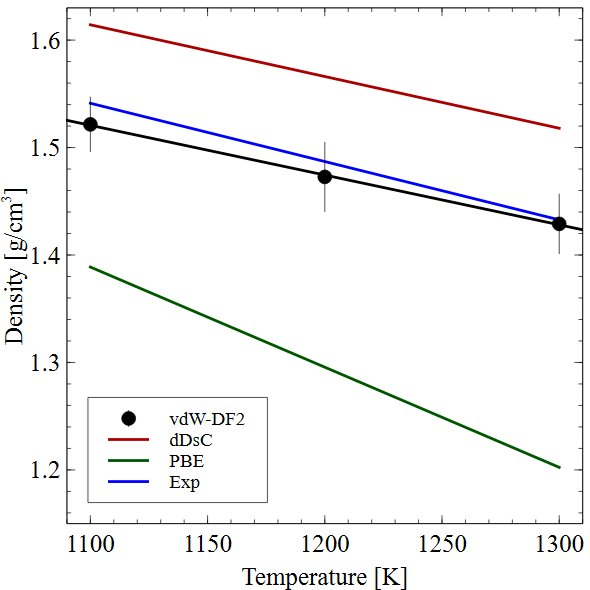
\includegraphics[width=0.7\textwidth]{NaCl-density.jpg} 
 \caption{The density of NaCl predicted with different dispersion models\cite{ANDERSSON2022153836} and compared to experimental correlation \cite{janz1988thermodynamic}.}
 \label{fig:NaCl_density}
\end{figure}

\begin{table}[h!]
\caption{Calculated correlations for density and heat capacity (C$_p$) of NaCl and PuCl$_3$. The temperature ranges are given for the range used to fit the AIMD simulations.}
\centering
\begin{tabular}{|c|c|c|c|}
\hline
                      & Density (g/cm$^{3}$) & C$_p$ (J/g-K)   & Temperature range (K)     \\
\hline
NaCl (vdW-DF2)        &  2.0301 - 0.0004630T             & 67.8 &  1100 - 1300  \\
NaCl (dDsC) \cite{ANDERSSON2022153836}        &  2.1338 - 0.0004814T                     & 69.0 &  1100  - 1500  \\
NaCl (Experiment)      & 2.1381 - 0.0005426T  \cite{janz1988thermodynamic}         &66.9 \cite{nist_ref}    & 1080 - 1300 \cite{janz1988thermodynamic} \\
PuCl$_{3}$ (vdW-DF2) &   5.0046 - 0.0006910T                   & 139.5 &    1100 - 1300 \\
PuCl$_{3}$ (dDsC)    &   5.4897 - 0.0009575T                   & 135.1 &    1100 - 1500   \\
PuCl$_3$ (DFT-D3)       &    5.5868 - 0.0009085T                  & 138.1 &   1100 - 1500 \\
\hline 
\end{tabular}
\label{table:rho_cp_correlation}
\end{table}

\subsubsection{Heat Capacity}
The isobaric heat capacity was calculated via Eq. \ref{eq:cp}, which utilizes the slope of the total energy with respect to temperature. The isobaric heat capacity was calculated for the vdW-DF2 functional and compared against experimental work \cite{nist_ref} and dDsC values reported by Andersson \cite{ANDERSSON2022153836}, all of which are provided in Table \ref{table:rho_cp_correlation}. The $R^2$ value for the heat capacity of NaCl calculated with the vdW-DF2 is 1.00. The simulations show a constant heat capacity with respect to the temperature, as has been previously observed with AIMD for molten salts \cite{duemmler_naclmgcl, karlsson2022synthesis, yuan2019specific, redkin2015heat}. There is excellent agreement with the literature for the isobaric heat capacity with a 1.36\% difference. 

\subsection{AIMD simulations of PuCl$_3$}
\subsubsection{Density and structure}
There is a complete lack of experimental data on the density of PuCl$_3$ for which to perform a computational validation. Thus, multiple dispersion formalisms were utilized to study PuCl$_3$ which have been shown to reasonably accurately reproduce properties of NaCl, UCl$_3$, and other chloride salt systems \cite{duemmler_liclkcl,duemmler_naclmgcl, ANDERSSON2022153836}. The primary dispersion formalism used to study PuCl$_3$ was the vdW-DF2 functional, with spot checks using the DFT-D3\cite{Grimme2010,grimme2011effect} and the dDsC \cite{steinmann2011comprehensive, steinmann2011generalized}. The density of PuCl$_3$ is shown in Fig. \ref{fig:pucl3_density} for all three dispersion formalisms. The vdW-DF2 predicts the smallest density while the DFT-D3 predicts the largest. It can also be seen that the vdW-DF2 predicts a different temperature dependence than the dDsC or DFT-D3 methods, which predict roughly the same temperature dependence. However, the differences in slope are likely not statistically significant. 

\begin{figure}[h!]
 \centering
 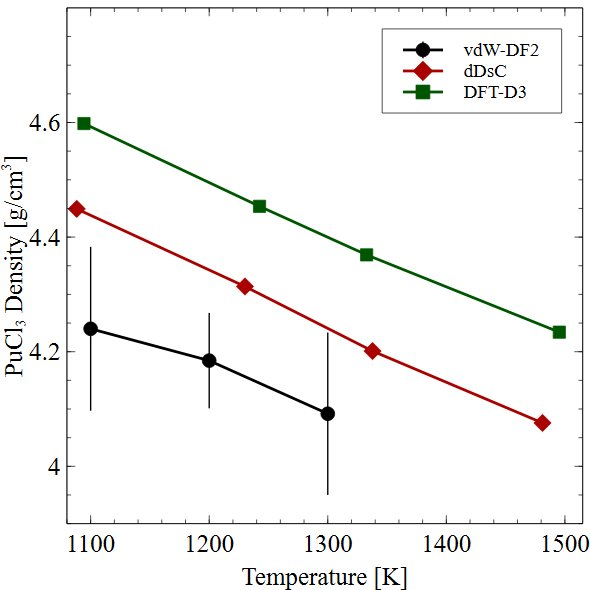
\includegraphics[width=0.7\textwidth]{PuCl-density.jpg} 
 \caption{The density of PuCl$_3$ as a function of temperature calculated with three different dispersion formalisms.}
 \label{fig:pucl3_density}
\end{figure}

The radial distribution function for PuCl$_3$ at 1300 K can be seen in Fig. \ref{fig:rdf_pucl3}. The Pu-Cl distance is observed to be at 2.90 {\AA}, which is a larger value than the values calculated via a DFT SVWN5 local functional approximation at 0 K (2.560 and 2.574 {\AA} \cite{buz2012dft}). It is expected that predictions of first neighbor distances would be shorter for calculations at 0 K, however, there are no experimental data with which to compare. For completeness, the Pu-Pu and Cl-Cl peaks were observed at 4.90 and 3.70 {\AA}, respectively. 

\begin{figure}[h!]
 \centering
 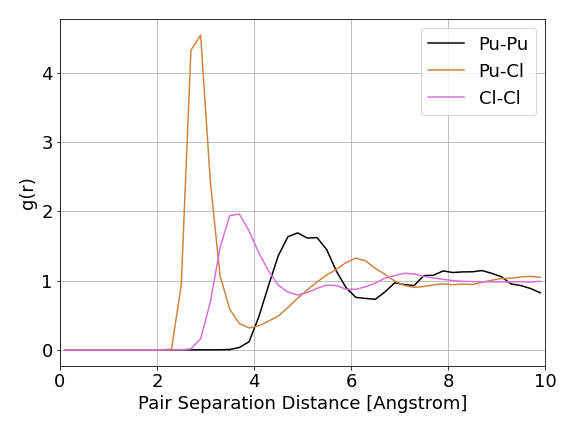
\includegraphics[width=0.7\textwidth]{rdf_pucl3_1300K.png} 
 \caption{The radial distribution function of PuCl$_3$ at 1300 K.}
 \label{fig:rdf_pucl3}
\end{figure}

\subsubsection{Heat Capacity}
The reported values of isobaric heat capacity were calculated from the slope of the total energy with respect to the temperature. The dependence of total energy follows a linear relationship with temperature and as a result, the reported value of heat capacity is constant with respect to the temperature over the range in this study. The isobaric heat capacities were studied for the vdW-DF2 dispersion functional, as well as the dDsC and DFT-D3 dispersion correction, and are shown in Table \ref{table:rho_cp_correlation}. The $R^2$ value for the vdW-DF2 formalism was 1.00. Once again, there is no experimental data available for comparison for the PuCl$_3$ system. 

\subsection{AIMD simulations of NaCl-PuCl$_3$}
\subsubsection{Density and structure}
The vdW-DF2 and dDsC dispersion formalisms were utilized to explore mixtures in the NaCl-PuCl$_3$ system. The density for the NaCl-PuCl$_3$ system is shown in Fig. \ref{fig:density} where it can be observed that the dDsC method predicts a larger value for density at all compositions than the vdW-DF2 functional. The solid lines in Fig. \ref{fig:density} are the first order (n=2) Redlich-Kister expansion for densities that are a function of temperature and composition. The fitting parameters can be seen in Table \ref{Table:RK_fit}. A Redlich-Kister expansion fitting was not performed for the dDsC, as it was only applied to a single temperature, 1250 K. The density calculated by the ideal mixing approach (Eq. \ref{eq:mixing}) is in excellent agreement with the AIMD results for for the densities. The Redlich-Kister expansion was used to describe the less than 1.5\% deviation that was observed and provide continuous interpolation between compositions and temperatures.
\begin{figure}[h!]
 \centering
 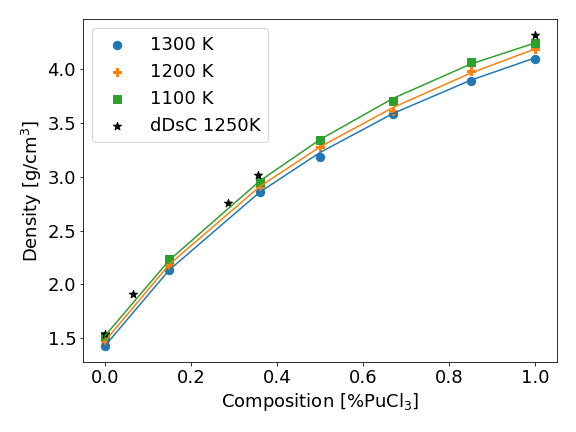
\includegraphics[width=0.7\textwidth]{Redlich_Kister.png} 
 \caption{Density of the NaCl-PuCl$_3$ system calculated with vdW-DF2 functional and dDsC at 1250 K. A first-order Redlich-Kister expansion density is plotted as solid lines.}
 \label{fig:density}
\end{figure}

\begin{table}[h!]
\centering
\caption{The fitting parameters ($A_1$, $A_2$, $B_1$, and $B_2$) for the first-order Redlich-Kister expansion for the density with the vdW-DF2 functional used in Eq. \ref{eq:Ln} and Eq. \ref{eq:RK}}
\begin{tabular}{|c|c|c|}
\hline
  & n=1           & n=2           \\
\hline
A$_n$ & -0.6769 & 1.3938  \\
B$_n$ & 4.5305E-4  & -1.0491E-3 \\
\hline
\end{tabular}
\label{Table:RK_fit}
\end{table}

The deviation from ideal mixing is shown in Fig. \ref{fig:deviation}. The ideal mixing is negative for the entire compositional space, within the limits of statistical certainty. The negative deviation from ideal mixing increases as the composition approaches the eutectic point of 36\% PuCl$_3$. Subsequently, as the PuCl$_3$ content in the mixture increases, there is a drive back toward an ideal mixing type behavior. Data points are actually slightly positive for the 80\%PuCl$_3$ composition, however, this is not considered a statistically significant result. There are limitations for converging a mixed salt system that would limit the accuracy to having an error of less than 1\% for the absolute density which causes some scatter in the collected data \cite{ANDERSSON2022153836}. Additionally, this largely conforms to the previous study on the NaCl-UCl$_3$ system, which showed variable deviation from ideal mixing as a function of composition, with a minimum near the eutectic composition \cite{ANDERSSON2022153836}. 

\begin{figure}[h!]
 \centering
 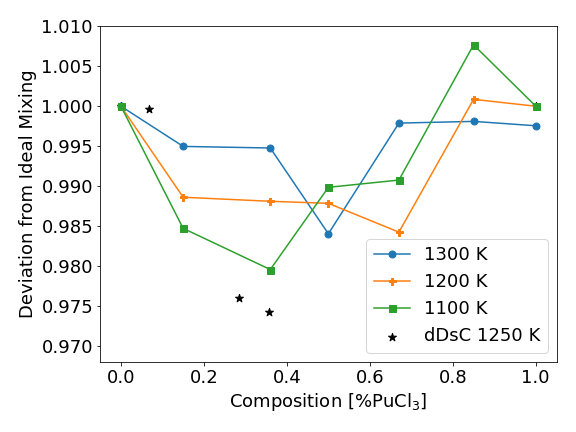
\includegraphics[width=0.7\textwidth]{Diviation_from_ideal_mixing.png} 
 \caption{Fractional deviation from the ideal solution behavior plotted from 1100 to 1300 K for the vdW-DF2 functional and 1250 K for the dDsC.}
 \label{fig:deviation}
\end{figure}

A direct comparison of density with literature is carried out on the eutectic composition and shown in Fig. \ref{fig:eutectic_density}. The experimental density from Karlsson et al. \cite{karlsson2022synthesis} is shown as red squares and a linear fit extrapolated to higher temperatures as a dashed red line, which are compared to three different vdW formalisms (the vdW-DF2, DFT-D3, and dDsC). The DFT-D3 overpredicts the density when compared with the experiment, which is expected as this occurs in other molten salts as well \cite{duemmler_liclkcl, duemmler_naclmgcl}. It can be observed that the dDsC is in excellent agreement at all temperatures below 1250 K but over-predicts the extrapolation at 1500 K.  The predicted temperature trends are in excellent agreement with the experimental results. The vdW-DF2 predicts a different temperature trend so at lower temperatures it has a larger error than at higher temperatures but still remains within 10\% of the experimental values. Generally, this is considered excellent agreement, and additional experiments are certainly warranted to confirm the existing computational and experimental work.

\begin{figure}[h!]
\centering
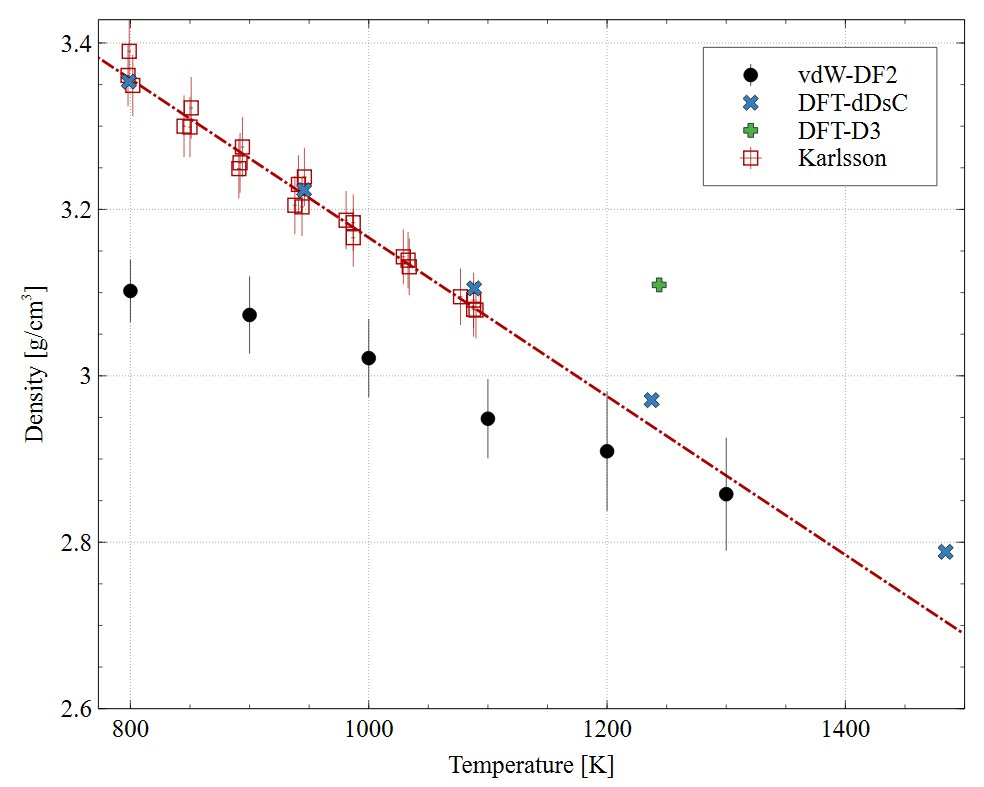
\includegraphics[width=0.7\textwidth]{density_comp.jpg}
\caption{The density of eutectic NaCl-PuCl$_3$ calculated with the vdW-DF2 functional and the dDsC compared against experimental results \cite{karlsson2022synthesis}.}
\label{fig:eutectic_density}
\end{figure}

\subsubsection{Coefficient of thermal expansion}

The coefficient of thermal expansion (CTE) is an important thermophysical property for nuclear applications as this influences the Doppler coefficient which will affect the moderation ratio and the reactivity in the core. The CTE was calculated using Eq. \ref{eq:CTE} and is shown in Fig. \ref{fig:CTE}. The minimum $R^2$ value occurred in the 50\%PuCl$_3$ system and was 0.925, the remaining values were above 0.97, indicating excellent linearity of the volume expansion with temperature, and thus a temperature-independent CTE. The CTE stays fairly constant with respect to the concentration, with minor fluctuations between 2$\times10^{-4}$ and 3$\times10^{-4}$ K$^{-1}$, and a minor general decreasing trend with increasing PuCl$_3$. There is also reasonable agreement with the literature \cite{karlsson2022synthesis} at the eutectic composition, albeit a slight underestimation. Generally, this is considered excellent agreement, and additional experimental data is warranted for a more refined analysis. 

\begin{figure}[h!]
 \centering
 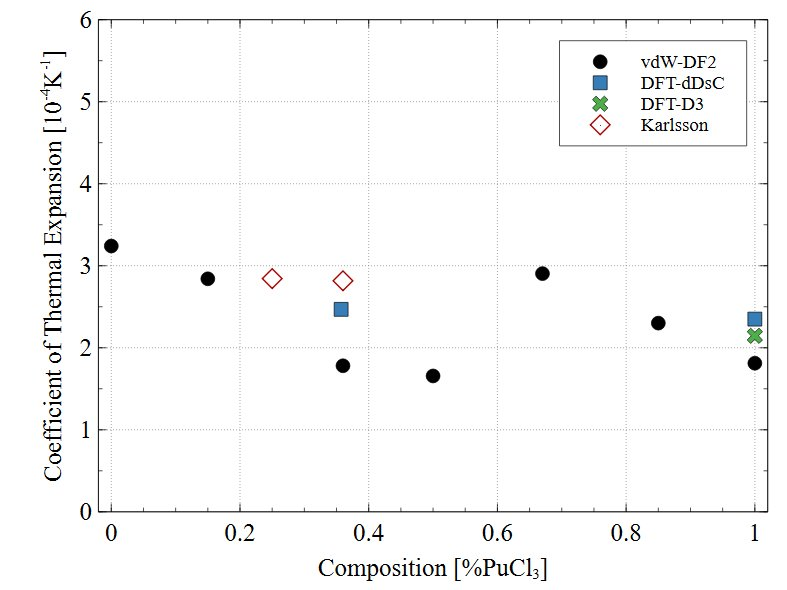
\includegraphics[width=0.7\textwidth]{CTE.jpg} 
 \caption{The coefficient of thermal expansion as a function of composition compared to the literature \cite{karlsson2022synthesis}.}
 \label{fig:CTE}
\end{figure} 

\subsubsection{Heat capacity and mixing enthalpy}

The isobaric heat capacities for the eutectic composition can be seen in Fig. \ref{fig:Cp_eut}. There are several things to note, first that the experimental studies do not agree with each other \cite{karlsson2022synthesis, lichtenstein2022property}. Lichtenstein et al. report an increasing heat capacity for 38.3 and 37.4 mol\% PuCl$_3$ while Karlsson et al. report a decreasing heat capacity with half the magnitude that Lichtenstein reported. In the Karlsson et al. study, they also conducted a brief AIMD study (closed green markers) which somewhat agrees with their experimental results. Our study agrees quite well with the experimental study of Karlsson et al. and their AIMD study, while it shows significant differences when compared to the results of Lichtenstein et al.

\begin{figure}[h!]
 \centering
 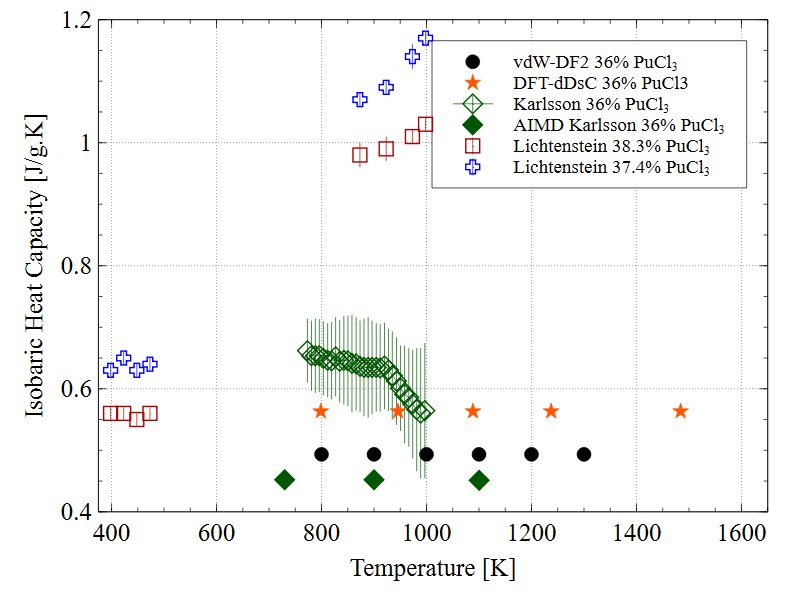
\includegraphics[width=0.7\textwidth]{Cp_eut.jpg} 
 \caption{The isobaric heat capacity for the eutectic composition compared against the available literature \cite{karlsson2022synthesis,lichtenstein2022property}.}
 \label{fig:Cp_eut}
\end{figure}

The compositional dependence of the isobaric heat capacity is shown in Fig. \ref{fig:Cp}. Similar to the pure NaCl and PuCl$_3$ species, the heat capacity is found to be constant over the observed temperature range. The magnitude of C$_p$ increases as the concentration of PuCl$_3$ increases in the system (in units of J/mol-K, an inverse relationship is observed if using units of J/g-K). The rate of increase is about 7.5 J/mol-K per 10 mol\% PuCl$_3$. To reiterate, only data for the eutectic composition is currently available in the literature. 

\begin{figure}[h!]
 \centering
 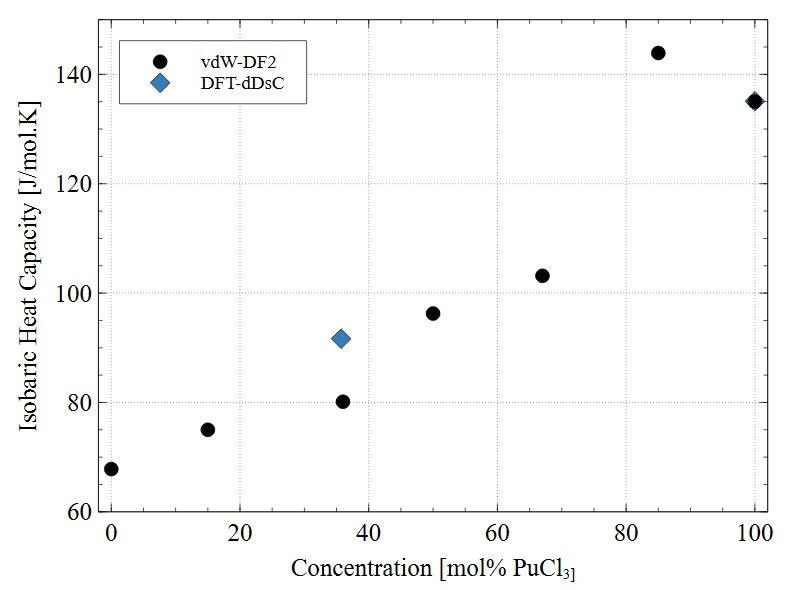
\includegraphics[width=0.7\textwidth]{Cp.jpg} 
 \caption{The isobaric heat capacity for NaCl-PuCl$_3$ as a function of composition.}
 \label{fig:Cp}
\end{figure} 

The enthalpy of mixing for NaCl-PuCl$_3$ mixtures can be seen in Fig. \ref{fig:mixing} which shows a parabolic function of composition. This holds true regardless of temperature or vdW formalism used. In all cases what can be observed is that the minimum value occurs near the eutectic composition, which is an expected behavior. In the case where vdW-DF2 was studied, there are no significant temperature trends that can be observed. There is excellent agreement with the enthalpy of mixing between the vdW-DF2 and the dDsC formalism. Once again there are no experimental values to compare against for enthalpy of mixing.

\begin{figure}[h!]
 \centering
 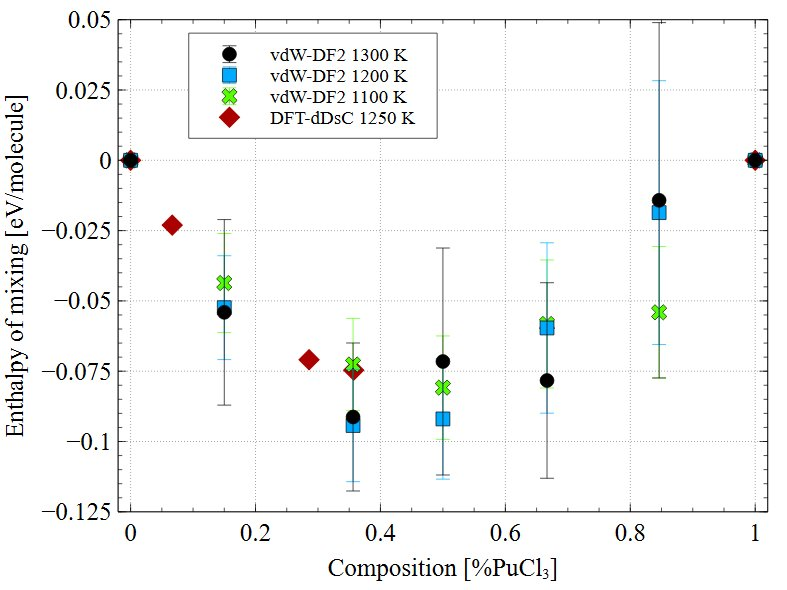
\includegraphics[width=0.7\textwidth]{mixing.jpg} 
 \caption{The enthalpy of mixing as a function of composition and temperature in NaCl-PuCl$_3$ mixtures calculated with the vdW-DF2 and dDsC dispersion formalisms.}
 \label{fig:mixing}
\end{figure} 


\FloatBarrier
\subsubsection{Compressibility}
The compressibility for NaCl-PuCl$_3$ can be seen in Fig. \ref{fig:compressibility}. The compressibility was calculated from the pressure as a function of the volume. Thus, each data point in Fig. \ref{fig:compressibility} represents 25 unique simulations consisting of five volumes and five unique velocity distributions at each volume. The general trend that can be observed is that the compressibility increases as the temperature increases. The compressibility of NaCl-PuCl$_3$ does not appreciably change with respect to composition. This same behavior was observed with NaCl-MgCl$_2$ \cite{duemmler_naclmgcl}. Neither is there a statistically significant temperature dependence for the compressibility of NaCl-PuCl$_3$. LiCl-KCl does observe composition dependence of the compressibility \cite{duemmler_liclkcl, Bengston2014}. The magnitude of the compressibility is similar to other molten salts, such as NaCl-MgCl$_2$ \cite{duemmler_naclmgcl} and LiCl-KCl \cite{duemmler_liclkcl, Bengston2014}. There is no experimental data available for comparison. 
\begin{figure}[h!]
 \centering
 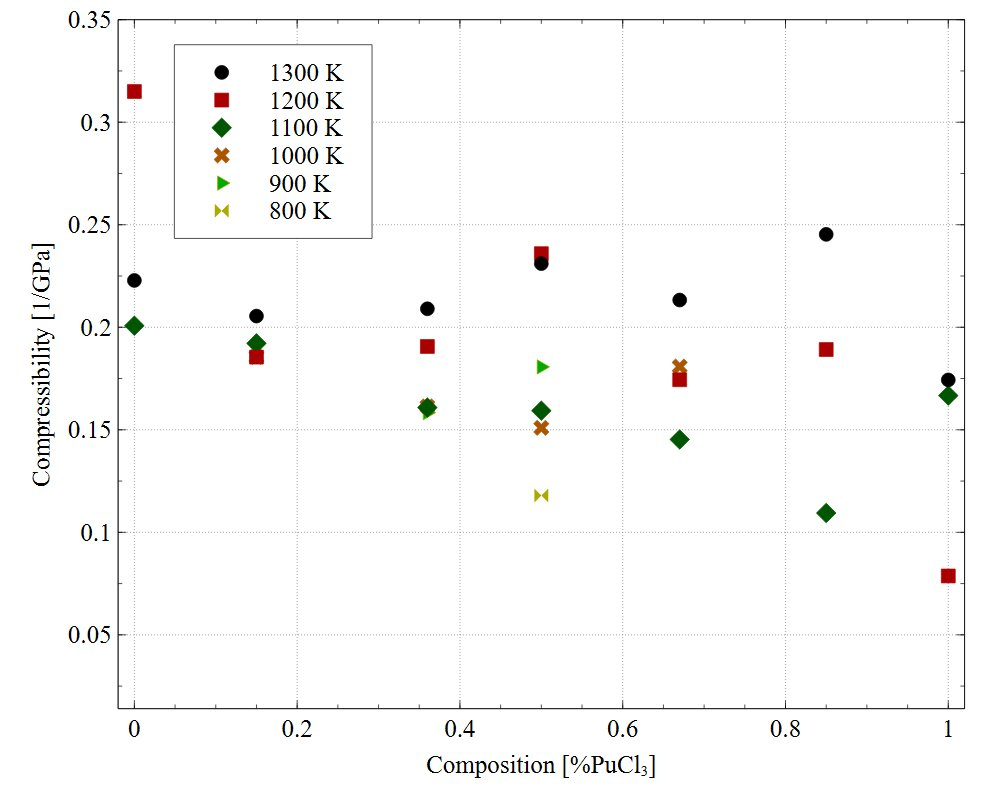
\includegraphics[width=0.7\textwidth]{compressibility_no_fits.jpg} 
 \caption{The calculated compressibility for the NaCl-PuCl$_3$ pseudo-binary system as a function of composition at six different temperatures.}
 \label{fig:compressibility}
\end{figure} 
\FloatBarrier

\section{Discussion}
This discussion will focus on the local structural behavior of mixtures of NaCl and PuCl$_3$ salts. Fig. \ref{fig:rdf_comp} plots the pair distribution function of NaCl and five salt mixtures at different compositions (x=0.15, x=0.36, x=0.50, x=0.67, x=0.85) at 1300 K including a comparison with the radial distribution function of pure PuCl$_3$ at 1300 K.

\begin{figure}[h!]
 \centering
 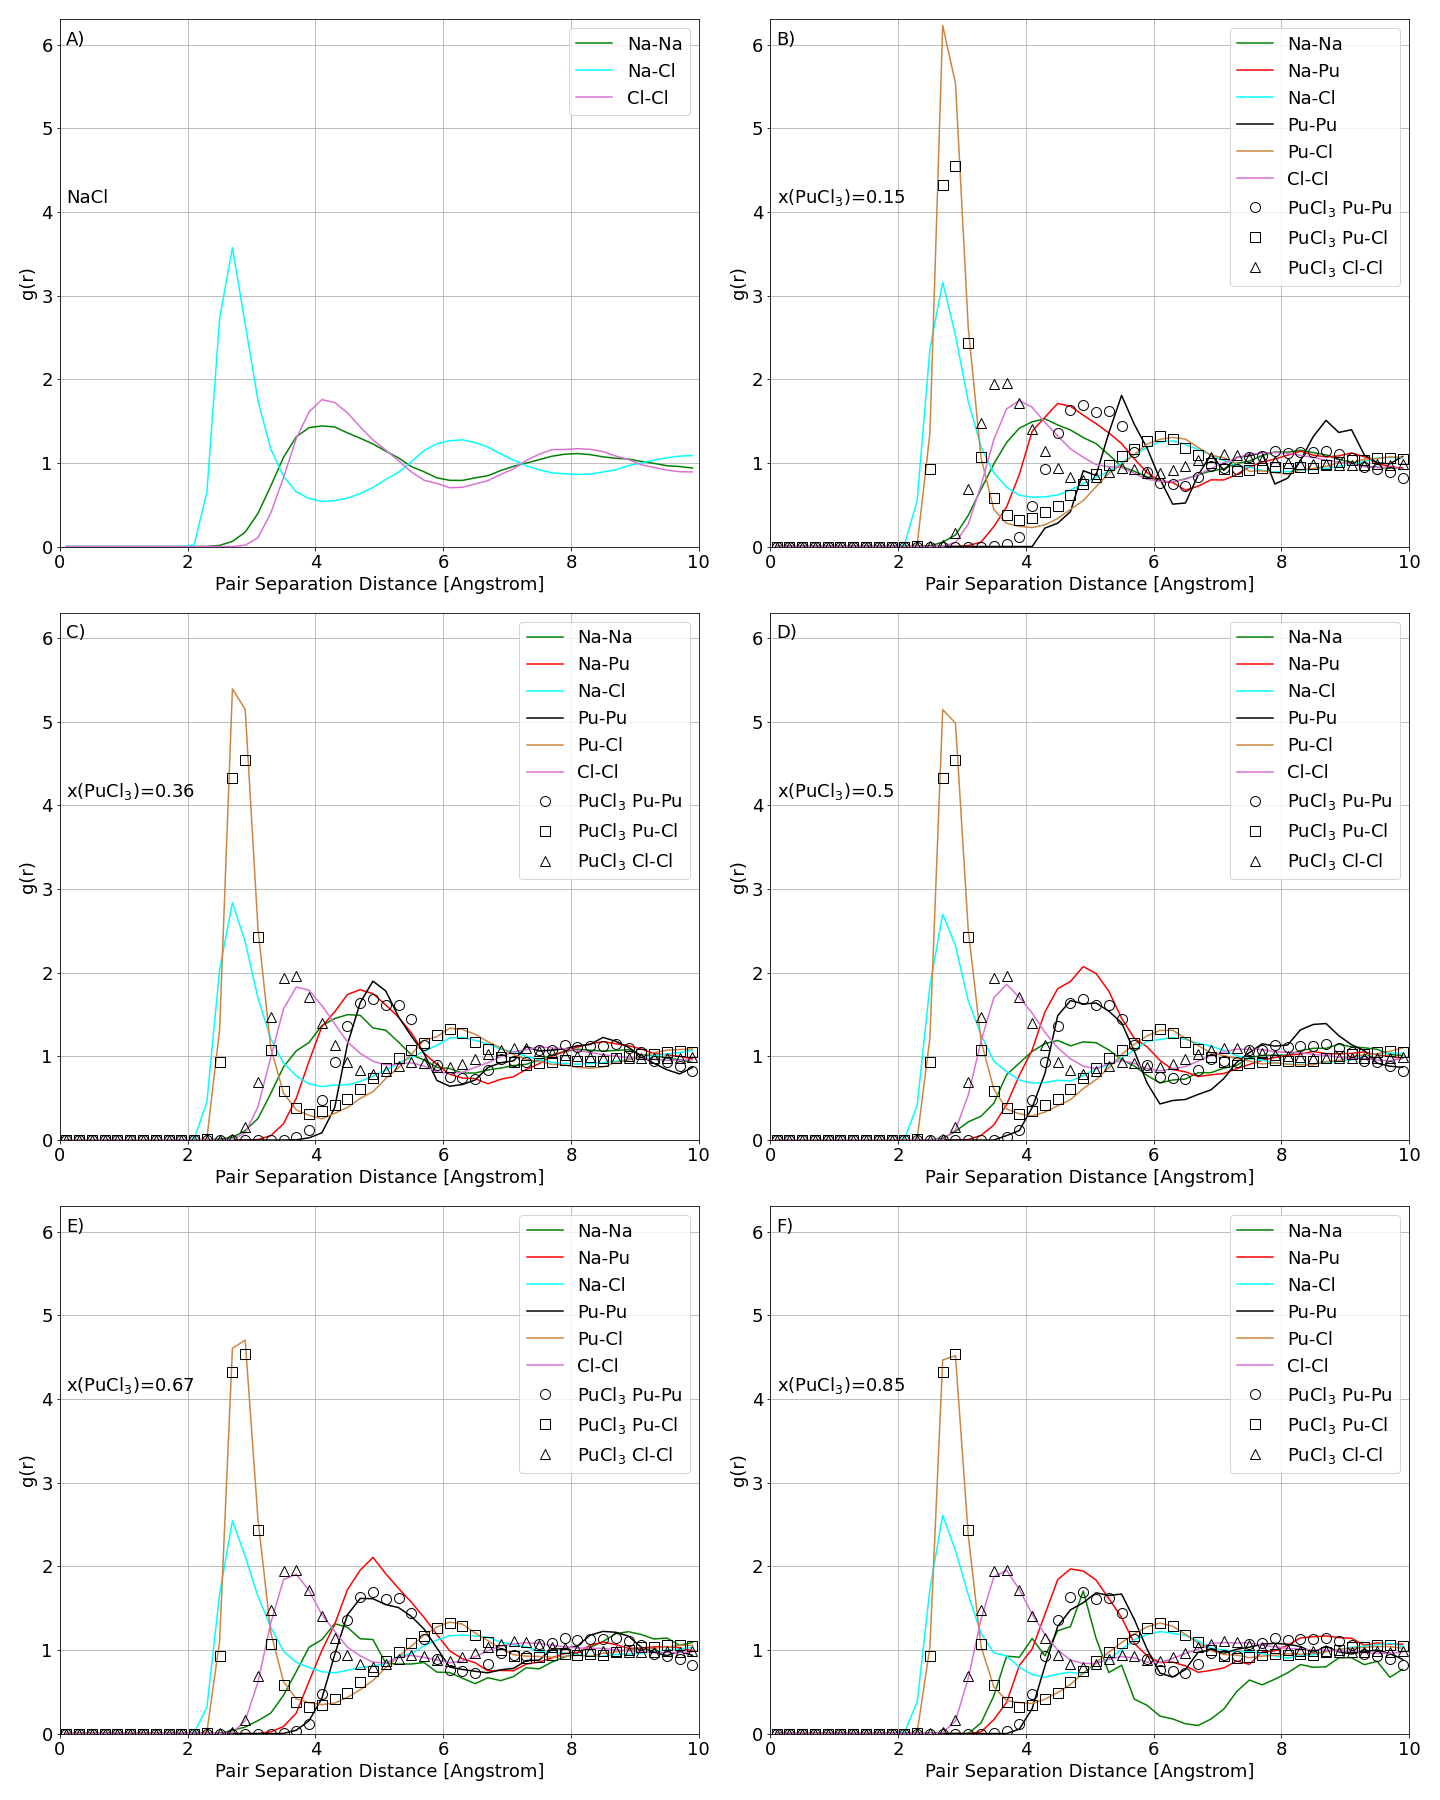
\includegraphics[width=\textwidth]{rdf_comp_to_pucl3.png} 
 \caption{Pair distribution function at 1300 K of NaCl-PuCl$_3$ as a function of composition (x = 0, 0.15, 0.36, 0.50, 0.67, 0.85). The reference functions are Pu-Cl and Pu-Pu bond from the pair distribution of PuCl$_3$. }
 \label{fig:rdf_comp}
\end{figure} 

The molten salt NaCl-UCl$_3$ has been identified to create networks when the concentration of UCl$_3$ increases above 30\% and also in localized cases below that concentration \cite{li2019first}. This appears to be the case with NaCl-PuCl$_3$ as well. Based on the behavior exhibited by the pair distribution function (Fig. \ref{fig:rdf_comp}) we observe that the Pu-Pu bond is almost identical to that of pure PuCl$_3$ when considering both the shape and the amplitude of the curve for all concentrations above 36\%. The eutectic concentration has the same peak distance but the amplitude is larger than what is observed in pure PuCl$_3$ for the Pu-Pu bond. This suggests that the cutoff for network formation is between 15\% and the eutectic value of 36\%, which falls in the same range observed in NaCl-UCl$_3$ \cite{ANDERSSON2022153836}. In Fig. \ref{fig:rdf_comp}b, there is a shift in both the position and the amplitude of the Pu-Pu bond which suggests that at this concentration (15\% PuCl$_3$) the mixture is unable to maintain the network structure. It must be noted that with small simulation cells as presented here, it is challenging to make strong claims, and an expansive study would be necessary for the express purpose of network formation and analysis, which is not in the scope of this study. 

The Pu-Pu coordination number as a function of PuCl$_3$ composition at 1300 K is displayed in Fig. \ref{fig:coordination_number} and was calculated by integrating the radial distribution function to the first minimum after the maximum, as shown in Eq. \ref{eq:CN}. This figure shows that the Pu-Pu coordination number increases in a linear fashion with respect to the concentration of PuCl$_3$. The only concentration that deviates from this linear increase is 67\% PuCl$_3$. The overall trend of linearly increasing Pu-Pu coordination with increasing Pu content was also observed at 1100 K and 1200 K. However, the deviation at 67\% is not observed at the other temperatures. The coordination number is not influenced by the temperature which, in combination with similar behavior on the radial distribution functions, would suggest that no temperature dependence in the structural mechanisms, like network formation, is observable.

\begin{figure}[h!]
 \centering
 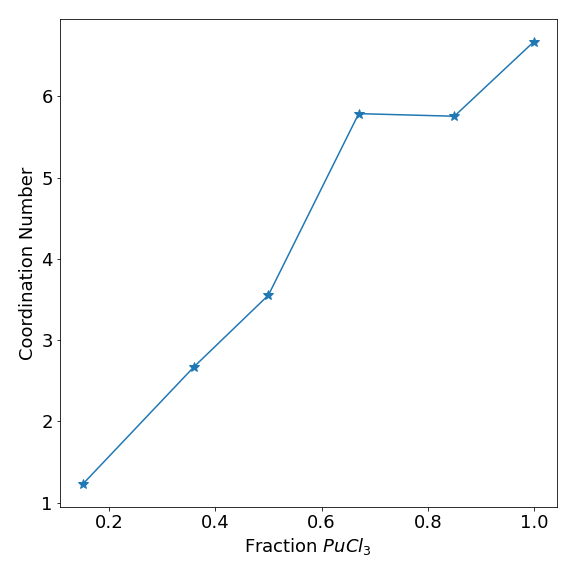
\includegraphics[width=0.7\textwidth]{coordination_number.png} 
 \caption{Pu-Pu coordination number in NaCl-PuCl$_3$ as function of composition at 1300 K.}
 \label{fig:coordination_number}
\end{figure}

The concentrations with the largest deviations from ideal mixing occur at 15\% and 36\% PuCl$_3$ (Fig. \ref{fig:deviation}), which corresponds to the concentrations where there is a transition from partial phase separation or partial networking to a network-dominated structure. A similar observation can be observed in the NaCl-UCl$_3$ system \cite{ANDERSSON2022153836}.
\

\FloatBarrier

\section{Conclusions}
This work calculated the thermophysical properties of NaCl-PuCl$_3$ for seven unique compositions through \textit{ab initio} molecular dynamics. The literature on plutonium-bearing salts is extremely limited. The densities predicted by the vdW-DF2 functional agree well with the literature, showing excellent agreement with NaCl and slightly underestimating the eutectic density. The dDsC dispersion correction showed excellent agreement with experiments for the eutectic compositions. A first-order Redlich-Kister expansion has been applied to the density to account for the 2\% deviation from ideal mixing that is observed with this salt. Both vdW-DF2 and the dDsC show excellent agreement with the magnitude of experimentally determined heat capacities, though there is disagreement among both experiments and computational predictions regarding the trends of the heat capacity with temperature. Coordination analysis indicates that network formation is observed in the PuCl$_3$-rich concentrations and is prevalent in all concentrations above 36\%. This study provides an in-depth study of the thermophysical and structural properties of the pseudo-binary salt NaCl-PuCl$_3$ and can serve to inform thermophysical databases, computational fluid dynamics studies, and thermochemical modeling.

\section{Acknowledgements} 

This material is based upon work supported under a University Nuclear Leadership Program Graduate Fellowship. This work is also supported through the INL Laboratory Directed Research and Development (LDRD) Program under DOE Idaho Operations Office Contract DE-AC07-05ID14517. This research made use of the resources of the High-Performance Computing Center at Idaho National Laboratory, which is supported by the Office of Nuclear Energy of the U.S. Department of Energy and the Nuclear Science User Facilities.  

This work was partially sponsored by the Los Alamos National Laboratory Directed Research and Development (LDRD) program and used resources provided by the Los Alamos National Laboratory Institutional Computing Program. Los Alamos National Laboratory, an affirmative action/equal opportunity employer, is operated by Triad National Security LLC, for the National Nuclear Security Administration of the U.S. Department of Energy under Contract No. 89233218CNA000001.

\FloatBarrier


\bibliography{references}
%\end{multicols}
\end{document}
